
%(BEGIN_QUESTION)
% Copyright 2010, Tony R. Kuphaldt, released under the Creative Commons Attribution License (v 1.0)
% This means you may do almost anything with this work of mine, so long as you give me proper credit

Identify the regular operating conditions of these solenoid valves so that they form a {\it 1oo2 trip} system, where only one solenoid needs to ``trip'' from its regular operating state to move the control valve:

$$\includegraphics[width=15.5cm]{i01358x01.eps}$$

Near each solenoid, place the label ``NE'' (normally energized) or ``NDE'' (normally de-energized) as your answers to this question.

\underbar{file i01358}
%(END_QUESTION)





%(BEGIN_ANSWER)

$$\includegraphics[width=15.5cm]{i01358x02.eps}$$

%(END_ANSWER)





%(BEGIN_NOTES)

{\bf This question is intended for exams only and not worksheets!}.

%(END_NOTES)

